\onehalfspacing
\section{Konzept}
Zu Beginn der Konzeptionsphase werden die Anforderungen an das Projekt definiert. Hierzu werden Absprachen mit dem Auftraggeber getroffen, sowie die bereits vorhandenen Testfälle anderer Projekte analysiert. Aus den daraus erhaltenen Informationen wird im Anschluss eine Anforderungsdefinition erstellt. Nachdem die Anforderungen an das Projekt definiert sind, folgt die Entwicklung einer geeigneten Softwarearchitektur.
\subsection{Analyse bisheriger Testfälle}
Zur Ermittlung der Testfälle, welche durch die Suite abgedeckt werden sollen, werden die bisherigen Testpläne analysiert. Schwierigkeit hierbei ist, dass der Geber vor ca. 20 Jahren entwickelt wurde. Zum Entwicklungszeitpunkt fand keine, den heutigen Standards entsprechende, Dokumentation der Testfälle (Testplan) statt. Weiterhin ist zum Projektstart noch kein Testplan für die Portierung des Controllers vorhanden. Aus diesem Grund wird für die Analyse der Testfälle auf den Testplan eines ähnlichen Produktes (SEY) zurückgegriffen. Der SEY eignet sich hier, da er ebenfalls über eine Hiperface Schnittstelle verfügt.\newline
Die im Testplan festgelegten Tests werden in eine Excel Tabelle übertragen. Die Testfälle sind im Testplan in verschiedene Kategorien unterteilt (zum Beispiel General Requirements, HW Architecture, Functional Requirements). Im Unterschied zum SK verfügt der SEY über zwei Mikrocontroller (Master und Slave, dies führt dazu das einige Testfälle im Testplan doppelt vorhanden sind. Da diese Dopplung für den SKx nicht notwendig ist werden zu Beginn der Analyse die entsprechenden Dopplungen entfernt. In einem zweiten Schritt wird die Beschreibung jedes Testfalls analysiert. Die Beschreibung der Testfälle erfolgt in Textform. Jeder Testfall ist durch eine Testfallnummer (zum Beispiel SW00077) eindeutig identifizierbar. Bei der Analyse werden die Kriterien aus \dq \nameref{tab:KriterienAuto}\dq~angewendet. Hierdurch wird geprüft ob ein Testfall unter den derzeit gegebenen Rahmenbedingungen des Projekts Automated Testing @ GBC07  realisierbar ist. Ein Beispiel für einen nicht automatisierbaren Testfall ist zum Beispiel beim Eingriff mittels Debugger während des Tests gegeben. Als Ergebnis der Bewertung stehen drei Auswahlmöglichkeiten zur Verfügung (gegeben, nicht gegeben, mit Änderungen). Das Ergebnis \dq mit Änderungen\dq~dient dazu, Testfälle zu identifizieren welche im Moment zum Beispiel aufgrund fehlender Hardware am Teststand nicht realisierbar sind, zu identifizieren. Bei diesen Testfällen wäre eine spätere Realisierung in einer weiteren Ausbaustufe des Teststandes möglich.

\begin{table}[h]
\begin{center}
\begin{tabularx}{\textwidth}{|c|X|X|c|}
\hline
\rowcolor{cyan} & Nummer des Tests aus Testplan: & & SW000016  \\
\hline
\rowcolor[gray]{0.6} Anford. Nr. & Anford. Bezeichnung & Beschreibung & Bewertung \\
\hline
01 & Externe Software & Externe Software wie zum Beispiel der Einsatz eines Debuggers darf nicht gefordert werden & \cellcolor{green}gegeben \\
\hline
02 & Timing Test & Zeitmessungen sind aufgrund der nicht Echtzeitfähigen BS schwer zu realisieren & \cellcolor{green} gegeben \\
\hline
03 & Manueller Eingriff & es darf kein manueller Eingriff in den Test (zum Beispiel umstecken, auslesen eines Registers, Prüfungen direkt im Quellcode) notwendig sein
 & \cellcolor{red} nicht gegeben \\
\hline
04 & Externe Hardware & Für den Test benötigte Hardware muss am Teststand vorhanden sein &\cellcolor{yellow} mit Änderungen \\
\hline
05 & Produkt spezifisch & Test ist auf spezielle Produkt Eigenschaft ausgelegt & \cellcolor{green}gegeben \\
\hline
\rowcolor[gray]{0.6} Ergebnis & & &\cellcolor{red} nicht bestanden \\
\hline
\end{tabularx}
\end{center}
\caption{Kriterien für Testauswahl \label{tab:KriterienAuto}}
\end{table}
\cleardoublepage

Aus der Analyse der Testfälle mittels \dq \nameref{tab:KriterienAuto}\dq~ergibt sich eine Gruppe von Testfällen, welche sich grundsätzlich zur Automatisierung unter den derzeitigen Gegebenheiten eignet. Die Gruppe beinhaltet hierbei eine Vielzahl verschiedener Tests (Hiperface Schnittstelle, Positionsbestimung, Power Supply Tests). Um eine bessere Übersicht zu erhalten, werden die Testfälle in Cluster gegliedert. Die Einteilung erfolgt in die sechs Kategorien Error Codes, Hiperface Commands, Position and external Sensors, Temperatur and Power Supply, Settings und Other. Um den weiteren Verlauf der Analyse- und Konzeptionsphase zu vereinfachen, werden im Anschluss die benötigten Hard- und Softwareschnittstellen für die verschiedenen Cluster identifiziert. Die Tabelle \dq \nameref{tab:Testcluster}\dq~zeigt beispielhaft die Cluster der  Tests, verschiedene Cluster sind hierbei farblich abgegrenzt. Die vollständige Tabelle befindet sich im Anhang.

\begin{table}[h]
\begin{center}
\begin{tabularx}{\textwidth}{|c|X|X|c|}
\hline
\rowcolor[gray]{0.6}
Test & Kategorie & Inhalt & Bemerkung \\
\hline
\rowcolor{cyan}
SW00001 &General Requirements & Firmware version format &  \\
\hline
\rowcolor{cyan}
SW00030 &HW Architecture & Master IcDSL IcDSL resolution is set by EEPORIM parameter Part 1 & \\
\hline
\rowcolor{cyan}
SW00031 &HW Architecture & Master IcDSL IcDSL resolution is set by EEPORIM parameter Part 2 &   \\
\hline
\rowcolor{cyan}
SW00058 &Functional Requirements & Boot-loader &  \\
\hline
\rowcolor{cyan}
SW00132 &Functional Requirements & General user cmds WEnterBootloader (70h) NO support of safety variants &  Nur für Safety Variante
\\
\hline
\rowcolor{red}
SW00017 &HW Architecture & Master mic. Supply Voltage Monitoring Part 1 (Accuracy) &  \\
\hline
\rowcolor{red}
SW00018 &HW Architecture & Master mic. Supply Voltage Monitoring Part 2 (Lower limit)
 &  \\
\hline
\rowcolor{red}
SW00021 &HW Architecture & Master mic. Internal Voltage Rail 1.8V
 &  \\
\hline
\rowcolor{green}
SW00078 &Functional Requirements & Error handlig referred to Hiperface specification 
 &  \\
\hline

\end{tabularx}
\end{center}
\caption{Testcluster \label{tab:Testcluster}}
\end{table}
\cleardoublepage


\subsection{Anforderungsdefinition}\label{sec:Anforderungsdefinition}
Eine klare Definition der Anforderungen an das Softwareprojekt dient im Verlauf dazu. die Endabnahme des Projekts zu erleichtern. Weiterhin werden durch die Anforderungen SMARTe \cite{Dr.WolfgangSchroder.2018} Ziele definiert, welche die weitere Projektstruktur positiv beeinflussen soll. 
Die während der Analyse erhaltenen Ergebnisse dienen hierbei als Grundlage für die Anforderungsdefinition. Weitere Anforderungen werden darüber hinaus durch den Auftraggeber (Betreuer der Ausbildungsfirma) vorgegeben.  Auf die Erstellung einer vollständigen \ac{SRS} wird im Rahmen dieses Projekt aus Zeitgründen bewusst verzichtet. Bei den Anforderungen wird zwischen funktionalen und nicht funktionalen unterschieden. Funktionale Anforderungen sind all jene, welche eine konkrete Funktion der Software definieren. Nicht funktionale Anforderungen sind Anforderungen wie zum Beispiel Zuverlässigkeit und Zeitverhalten. Die Anforderungen sind in den Tabellen \dq \nameref{tab:Anforderungstabelle}\dq~und \dq \nameref{tab:Anforderungstabelle2}\dq~dargestellt. Die Reihenfolge und Nummerierung der Anforderungen spiegeln gleichzeitig ihre Relevanz für das Projekt wieder.
\newpage
\begin{table}[h]
\begin{center}
\begin{tabularx}{\textwidth}{|c|X|X|c|}
\hline
Nr. & Bezeichnung & Beschreibung & Zuordnung \\
\hline
F01 &Integration in Automated Testing @ GBC07  & Die Suite muss in das Projekt Automated Testing @ GBC07 Integrierbar sein (Implementierung in ITE, Aufbau nach Vorgaben des Projekts) & Funktional \\
\hline
F02 & Schnittstellen Config & Auslesen und prüfen der Schnittstellen Parametrisierung und Funktionalität & Funktional \\
\hline
F03 & Diagnose Funktionalität & Überprüfung der vorhandenen Diagnose Funktionalität (zum Beispiel Spannungs Monitoring) & Funktional \\
\hline
F04 & Core Funktionalität & Prüfung der externen Temperatur Schnittstelle, sowie der single- und multiturn Positionsbestimmung & Funktional \\
\hline
F05 & Identifikation des DUT & Überprüfung der Firmware Version, des elektronischen Typenschilds auf Korrektheit & Funktional \\
\hline
F06 & Hiperface Befehle & Überprüfung der Funktion der verschiedenen Hiperface Befehle sowie der entsprechenden Antwort & Funktional \\
\hline
F07 & Error Codes & Eignung zur Stimulation der verschiedenen Fehlerfälle und  dadurch Produktion der entsprechenden Fehlermeldungen (01h-23h) & Funktional \\
\hline


\end{tabularx}
\end{center}
\caption{Anforderungen funktional \label{tab:Anforderungstabelle}}
\end{table}

\begin{table}[h]

\begin{center}

\begin{tabularx}{\textwidth}{|c|X|X|c|}

\hline
Nr. & Bezeichnung & Beschreibung & Zuordnung \\
\hline
NF01 & Externes Equipment & Möglichkeit zur Integration des am Teststand vorhandenen externe Equipment & Nicht Funktional \\
\hline
NF02 & Universell einsetzbar & Der Aufbau der Suite soll so gestaltet sein, dass diese auch zukünftig für die Portierung anderer (ähnlicher) Produkte genutzt werden kann & Nicht Funktional \\
\hline
NF03 & Coding Guidelines & Der Aufbau der Suite soll so gestaltet sein, dass diese auch zukünftig für die Portierung anderer (ähnlicher) Produkte genutzt werden kann & Nicht Funktional \\
\hline


\end{tabularx}
\caption{Anforderungen nicht-funktional \label{tab:Anforderungstabelle2}}
\end{center}
\end{table}
\cleardoublepage



\subsection{Softwarearchitektur}
Um die Anforderungen aus der vorherigen Anforderungsanalyse erfüllen zu können, bedarf es der Planung einer entsprechenden Softwarearchitektur. Hierzu werden die Ergebnisse aus der Anforderungsanalyse und der Analyse der Testfälle zusammengetragen. Das Resultat ist eine Beschreibung der benötigten Hard- und Softwareschnittstellen welche die Suite abdecken muss.  Diese gliedern sich in:
\begin{itemize}
	\item ICP Con (RS232 auf RS485 Converter)
	\item Motor 
	\item Schaltnetzteil
	\item Logging Funktion
\end{itemize}
Nachdem ein Überblick über die entsprechenden Softwarekomponenten geschaffen ist, werden die bisher verwendeten Skripte analysiert. Dies soll dazu dienen Softwarekomponenten zu identifizieren die für das aktuelle Projekt wiederverwendet werden können, sowie sich einen Überblick über die bisherige Softwarearchitektur zu erarbeiten.
Ein Beispiel der alten Architektur ist in Abbildung \dq \nameref{fig:Uebersicht_alt.jpg}\dq~dargestellt.
\begin{figure}[h]
  \centering
   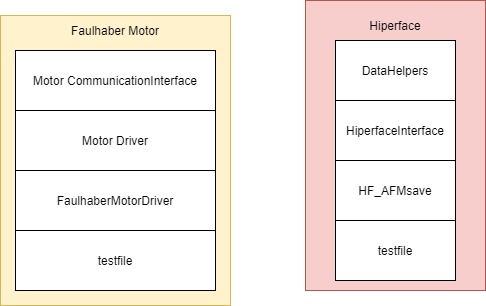
\includegraphics[width=1\textwidth]{img/Uebersicht_alt.jpg} 
   \caption{SW-Architektur HW Komponenten Alt}
   \label{fig:Uebersicht_alt.jpg}
\end{figure}
\cleardoublepage
Zu erkennen ist hierbei der schichtweise Aufbau der entsprechenden Module. Jedoch ergibt sich keine klare Softwarearchitektur, welche einheitlich auf die verschiedenen Komponenten angewendet werden kann. Die oberste Ebene jedes Testfalls wird durch das Testfile, welches die konkrete Implementierung des Testfalls enthält, gebildet. In den darunterliegenden Ebenen wird jeweils die Kommunikation mit den entsprechenden Hardwarekomponenten realisiert. Hierbei unterscheidet sich der architektonische Aufbau für die einzelnen Komponenten stark. Dies führt dazu, dass es für den Entwickler eines Tests sehr aufwendig ist zu prüfen welche konkreten Files bzw. Funktionen er für sein Testequipment nutzen muss. Weiterhin führt dieser Umstand dazu, dass die Testfallimplementierungen nur schwer für andere Tests mit anderen Hardware Anforderungen verwendet werden können.
\newline
Die Architektur der Suite soll es dem Benutzer ermöglichen die benötigten Hard- bzw. Softwarekomponenten einfach einzubinden. Weiterhin soll die Suite die Wiederverwendung der Testfallimplentierungen fördern.
Konkret ergeben sich also die folgenden Anforderungen an die Softwarearchitektur:
\begin{itemize}
	\item Erweiterbarkeit
	\item Einfache Wartbarkeit
	\item Benutzerfreundlichkeit
	\item Wiederverwendbarkeit
\end{itemize}
Um ein geeignetes Architekturmodell zu identifizieren werden drei Modelle verglichen. Als Modelle werden das MVC Pattern, das Pipe-Filter Modell und die Schichtenarchitektur gewählt. In Tabelle \dq \nameref{tab:vergleich}\dq~werden die Vor- und Nachteile der einzelnen Modelle bewertet, hierbei werden die Architekturen nach den Kriterien des aktuellen Projekt bewertet. Die Vor- und Nachteile können für andere Projekte variieren.
\newpage
\begin{table}[h]
\begin{center}
\begin{tabularx}{\textwidth}{|c|X|X|X|}
\hline
Kriterium & Pipe Filter & MVC & Schichten \\
\hline
Erweiterbarkeit & ++ & + & +++ \\
\hline
Wartung & +++ & ++ & +++ \\
\hline
Benutzerfreundlichkeit & + & +++ & +++ \\
\hline
Wiederverwendbarkeit & +++ & ++ & +++ \\
\hline


\end{tabularx}
\end{center}
\caption{Architekturmodelle im Vergleich  \label{tab:vergleich}}
\end{table}
Durch den Vergleich ergibt sich eine Schichtenarchitektur als geeignetes Modell. Die Schichtenarchitektur lässt in diesem Fall eine gute Abstraktion für den Benutzer zu, ohne das System zu komplex für eine Erweiterung bzw. Wartung zu machen. Hierdurch lässt sich auch das Prinzip von Kopplung und Kohäsion besser umsetzen. Als Herausforderung bei der Schichtenarchitektur zeigt sich die Auswahl der konkreten Anzahl Schichten. Hier wird eine drei-Schicht mit einer vier-Schicht Architektur verglichen. 
\begin{figure}[h]
  \centering
   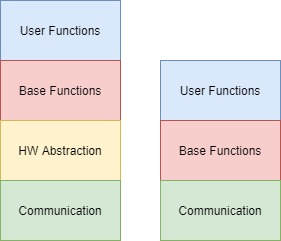
\includegraphics[width=0.75\textwidth]{img/VergleichSchichten.jpg} 
   \caption{Vergleich drei und vier Schichten}
   \label{fig:VergleichSchichten.jpg}
\end{figure}
Es zeigt sich, dass eine drei-Schicht Architektur prinzipiell möglich ist, jedoch gerade bei den Motor Modulen eine vier-Schicht Architektur für eine bessere Strukturierung und Trennung sorgt. Grund hierfür ist die Möglichkeit verschiedene Motoren mit jeweils unterschiedlichen Zusatzfunktionen nutzen zu können. Durch den zusätzlichen Hardware Abstraction Layer bei der vier Schicht Architektur lassen sich die unterschiedlichen Motoren besser abbilden.
Als unterste Schicht der Architektur wird die Communication Schicht gewählt. Diese übernimmt die Bereitstellung der entsprechenden Communication Interfaces. Als zweite Schicht wird eine Hardware Abstraktionsschicht eingeführt. Welche u.a die Treiber für die Hiperface Schnittstelle, sowie für die verschiedenen Motoren beinhaltet.
Die dritte Schicht (BaseFunctions) enthält die grundlegenden Befehle, welche zum Beispiel zum Starten eines Motors notwendig sind. Weiterhin enthält diese Schicht die Implementierung der grundlegenden Hiperfacebefehle. Die Userfunctions bilden die oberste Schicht der Architektur. Diese Schicht beinhaltet die Funktionalitäten, welche der Testentwickler für die konkrete Testfallimplementierung später benötigt. Beispiele hierfür sind z.B das auslesen des Typenschildes via Hiperface oder das Rotieren des Motors mit einen definierten Geschwindigkeit für eine gewisse Zeit. Der Nutzer der Suite kann also in Zukunft im Testverlauf einen Motor starten indem er die entsprechende Funktion der Suite aufruft, ohne dass er genaue Kenntnis über die konkrete Implementierung der Motortreiber oder geeigneter Motorfunktionen haben muss.
Neben den vier Schichten werden horizontal über alle vier Schichten hinweg zwei weitere Komponenten vorgesehen.
Zum Einen ist hier eine Klasse DataHelers welche, grundlegende Umrechnungsfunktionen sowie bestimmte globale Datenstrukturen enthält, vorgesehen. Zum anderen eine Klasse, welche die allgemeinen Testdaten speichert. Durch die horizontale Anordnung über alle Schichten hinweg ist ein Zugriff aus allen Schichten und Modulen auf diese Hilfsklassen möglich.
Als Besonderheit beim Architekturentwurf wird die Logging Funktion gesehen. Dies ist eine reine Softwarekomponenten und benötigt aus diesem Grund weder eine Communication noch eine Hardwareschicht. Durch die gewählte Schichtenarchitektur lässt sich aber auch dieser Fall gut realisieren.
Das Ergebnis dieses Grobentwurfs ist in Abbildung \dq \nameref{fig:SW_Arch_neu.jpg}\dq~dargestellt:
\begin{figure}[h]
  \centering
   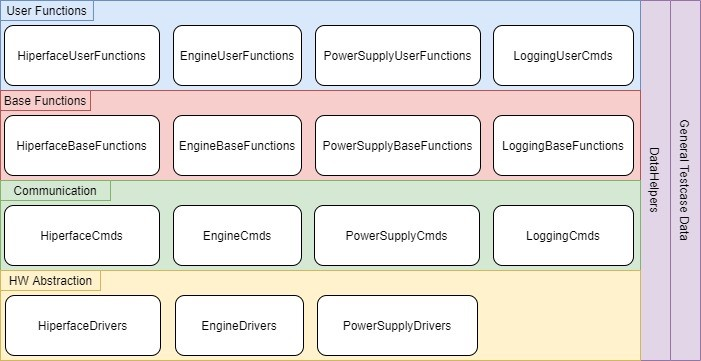
\includegraphics[width=1\textwidth]{img/SW_Arch_neu.jpg} 
   \caption{Softwarearchitektur Neu}
   \label{fig:SW_Arch_neu.jpg}
\end{figure}
\newpage
Die einzelnen Module der Software werden in den weißen Kästen dargestellt. Durch die hier entwickelte Architektur lassen sich die Module beliebig austauschen. Weiterhin ist die Architektur gut auf eventuelle spätere Erweiterungen übertragbar. 
Nach der Fertigstellung des Grobentwurfs erfolgt der Feinentwurf der Architektur. Hierzu werden für die einzelnen  Funktionalitäten jeweils Klassendiagramme angefertigt. Durch die angewendete Schichtenarchitektur lassen sich die Klassendiagramme einfach erstellen. Die Anzahl und Reihenfolge der Abhängigkeiten ist  beschränkt. In Abbildung \dq \nameref{fig:Klassen_Hiperface.jpg}\dq~ist das Klassendiagramm der Hiperface Funktionalität vereinfacht dargestellt. Auf die Abbildung der Klassenvariablen wurde aus Übersichtsgründen hierbei verzichtet. Die Aufteilung der Klassen entspricht den Modulen der Softwarearchitektur im Schichtenmodell. Die oberste Ebene \dq HiperfaceUserFunctions\dq~stellt die Benutzerebene dar. In dieser werden nur Funktionalitäten implementiert, welche für den Benutzer direkt relevant sind. In der darunterliegenden \dq HiperfaceBaseFunctions\dq~Klasse befinden sich die verschiedenen Kommandos, welche durch die Hiperface Schnittstelle spezifiziert sind. Die \dq HiperfaceDrivers\dq~Klasse enthält alle Funktionen, welche zum senden und  empfangen der verschiedenen Kommandos benötigt werden. Dies ist zum Beispiel die Berechnung der Checksumme. Als unterste Ebene kommt das \dq HiperfaceComIterface\dq~zum Tragen. Dies stellt die Funktionalitäten für das initialisieren, öffnen und schließen der Schnittstelle zur Verfügung.\newline
\begin{figure}[h]
  \centering
   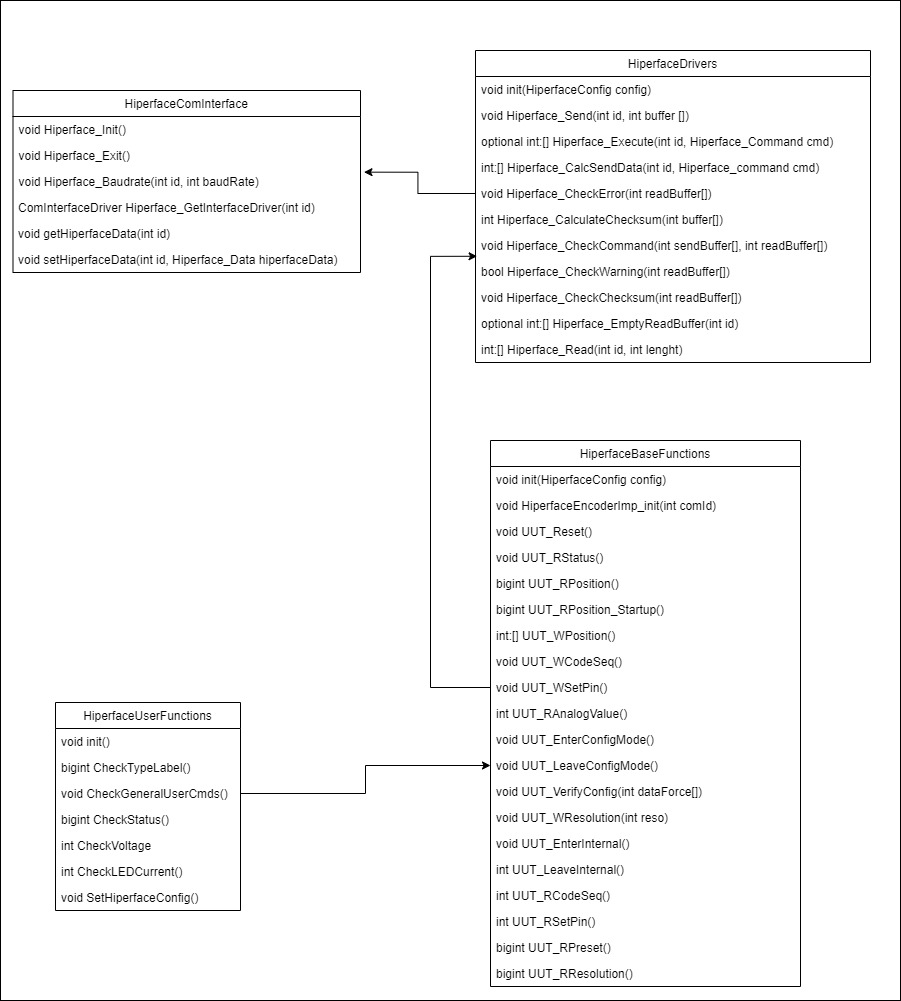
\includegraphics[width=1\textwidth]{img/Klassendiagramm_Hiperface.jpg } 
   \caption{Klassendiagramm Hiperface Neu}
   \label{fig:Klassen_Hiperface.jpg}
\end{figure}

Als Grundlage für die Konzeption der neuen Architektur dient eine bisherige Implementierung der Hiperface Schnittstelle. Diese ist in Abbildung \dq \nameref{fig:Klassen_Hiperface_Alt.jpg}\dq~zu sehen. Beim Vergleich der beiden Architekturen fällt auf, dass durch die neue Architektur eine deutlich bessere Abstraktion für den Benutzer erzielt wird. Weiterhin ist es mithilfe der neuen Architektur deutlich einfacher das Programm um weitere Module zu ergänzen, da einheitliche Schnittstellen geschaffen werden.
\begin{figure}[h]
  \centering
   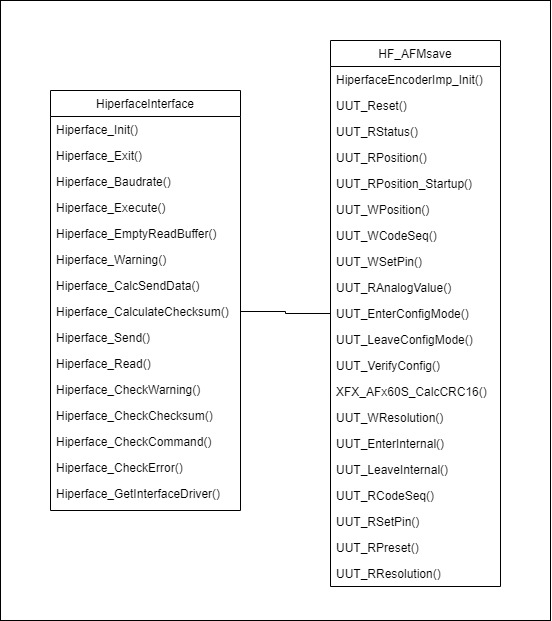
\includegraphics[width=1\textwidth]{img/Klassendiagramm_Hiperface_alt.jpg} 
   \caption{Klassendiagramm Hiperface Alt}
   \label{fig:Klassen_Hiperface_Alt.jpg}
\end{figure}
\cleardoublepage
Zum Zeitpunkt dieser Arbeit sind am Teststand zwei verschiedene Arten von Motoren vorhanden. Hierbei handelt es sich um einen Motor der Marke Faulhaber, sowie einen der Marke Metronix. Zwar sind die Basisbefehle dieser Motoren identisch, jedoch verfügen beide über dasselbe Kommunikationsinterface und dieselben Grundfunktionalitäten. Jedoch besitzen sie verschiedene, spezielle Befehle wie etwa das Setzen eines Operationsmode oder das Spezifizieren der Beschleunigung. Aufgrund dieser Unterschiede gestaltet sich die Erstellung der Driverschicht hier aufwendiger. Das \dq EngineDriver\dq~Modul gliedert sich in die drei Bestandteile \dq EngineDriver\dq, \dq MetronixEngineDriver\dq~und \dq FaullhaberEngineDriver\dq. Die Klasse \dq EngineDriver\dq~stellt die Grundfunktionalitäten bereit, von welcher die beiden spezifischen Motoren dann abgeleitet werden. 

\subsection{Wirtschaftlichkeit}
Im Rahmen des Projektmanagements wird weiterhin eine wirtschaftliche Betrachtung des Projekts versiert. Diese gestaltet sich jedoch aufgrund der mangelnden Datenlage schwierig. Die Kosten des Projektes werden durch die benötigte Arbeitszeit definiert. Weitere Kosten zum Beispiel für Hardwarekomponenten sind vernachlässigbar, da es sich bei der Testsuite um eine reine Softwarelösung handelt. Zwar wird das Projekt im Rahmen einer Bachelorarbeit bearbeitet, jedoch sind keine Angaben zu den Kosten eines Bacheloranten pro Stunde vorhanden. Aus diesem Grund wird für die Berechnung auf den in der Softwareentwicklung für solche Projekte vorgegeben Stundensatz von 90\euro{} angenommen und halbiert. Durch die Vorgabe der DHWB, welche einen Stundenaufwand von mindestens 360 Stunden für eine Bachelorarbeit vorsieht, ergeben sich daraus Kosten in Höhe von:
\begin{align*}
    45 \text{\euro} * 360 h {=} 16200 \text{\euro}
\end{align*}
Um beurteilen zu können ob das Projekt wirtschaftlich effizient ist, müssen diese Kosten nun mit den durch die Testsuite eingesparten Kosten zum Beispiel durch beschleunigte Testentwicklung etc. verglichen werden. Eine konkrete Abschätzung des durch die Testsuite reduzierten Aufwand, ist jedoch zu diesem Zeitpunkt nicht möglich. Es wird erwartet, dass die Zeitersparnis gerade in Bezug auf die in Zukunft kommenden Portierungen, das Projekt als wirtschaftlich darstellen wird. 




